\begin{figure*}
\centering
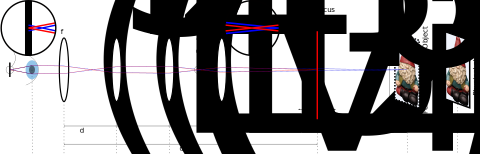
\includegraphics[width=0.89\textwidth]{images/varifocal_occlusion/unfolded}
%\fbox{\includegraphics[width=0.46\textwidth]{images/prototype}}
\caption[Varifocal-Occlusion: unfolded optics]{Illustration of the unfolded optical path of a 4-lens system for image-forming occlusion-capable AR displays. With a varifocal display, the distance of virtual image and occlusion mask matches the user's focus distance, indicated by the thick vertical red line. Red and blue lines going from points in the scene through the optics onto the retina indicate ray diagrams for the image formation of the virtual/occlusion image and for physical objects, respectively. Enlarged inset at the occlusion SLM shows that the physical world at the user's focus plane is brought into focus at the SLM where portions of the real world can be occluded. Enlarged inset at the retina shows that the same rays (red) that are in-focus at the occlusion SLM are also in-focus at the retina -- this property is utilized to also depict a perceptually correct occlusion mask for out-of-focus virtual objects by applying a computational blur. Finally, the image of real-world objects seen through the display should ideally have the same magnification and distances from the eye as compared to seeing the real world without the display, i.e. $\frac{h_i}{h_o}=1$ and $e=0$. In our implementation, we are able to match the magnification, but not the distance.}
\label{fig:varifocal_occlusion:unfolded}
\end{figure*}
